\documentclass[11pt,a4paper]{report}
\usepackage[textwidth=37em,vmargin=30mm]{geometry}
\usepackage{calc,xunicode,amsmath,amssymb,paralist,enumitem,tabu,booktabs,datetime2,xeCJK,xeCJKfntef,listings}
\usepackage{tocloft,fancyhdr,tcolorbox,xcolor,graphicx,eso-pic,xltxtra,xelatexemoji}

\newcommand{\envyear}[0]{2025}
\newcommand{\envdatestr}[0]{2025-05-18}
\newcommand{\envfinaldir}[0]{webdb/2025/20250518/final}

\usepackage[hidelinks]{hyperref}
\hypersetup{
    colorlinks=false,
    pdfpagemode=FullScreen,
    pdftitle={Web Digest - \envdatestr}
}

\setlength{\cftbeforechapskip}{10pt}
\renewcommand{\cftchapfont}{\rmfamily\bfseries\large\raggedright}
\setlength{\cftbeforesecskip}{2pt}
\renewcommand{\cftsecfont}{\sffamily\small\raggedright}

\setdefaultleftmargin{2em}{2em}{1em}{1em}{1em}{1em}

\usepackage{xeCJK,xeCJKfntef}
\xeCJKsetup{PunctStyle=plain,RubberPunctSkip=false,CJKglue=\strut\hskip 0pt plus 0.1em minus 0.05em,CJKecglue=\strut\hskip 0.22em plus 0.2em}
\XeTeXlinebreaklocale "zh"
\XeTeXlinebreakskip = 0pt


\setmainfont{Brygada 1918}
\setromanfont{Brygada 1918}
\setsansfont{IBM Plex Sans}
\setmonofont{JetBrains Mono NL}
\setCJKmainfont{Noto Serif CJK SC}
\setCJKromanfont{Noto Serif CJK SC}
\setCJKsansfont{Noto Sans CJK SC}
\setCJKmonofont{Noto Sans CJK SC}

\setlength{\parindent}{0pt}
\setlength{\parskip}{8pt}
\linespread{1.15}

\lstset{
	basicstyle=\ttfamily\footnotesize,
	numbersep=5pt,
	backgroundcolor=\color{black!5},
	showspaces=false,
	showstringspaces=false,
	showtabs=false,
	tabsize=2,
	captionpos=b,
	breaklines=true,
	breakatwhitespace=true,
	breakautoindent=true,
	linewidth=\textwidth
}






\newcommand{\coverpic}[2]{
    % argv: itemurl, authorname
    Cover photo by #2~~(\href{#1}{#1})
}
\newcommand{\makeheader}[0]{
    \begin{titlepage}
        % \newgeometry{hmargin=15mm,tmargin=21mm,bmargin=12mm}
        \begin{center}
            
            \rmfamily\scshape
            \fontspec{BaskervilleF}
            \fontspec{Old Standard}
            \fontsize{59pt}{70pt}\selectfont
            WEB\hfill DIGEST
            
            \vfill
            % \vskip 30pt
            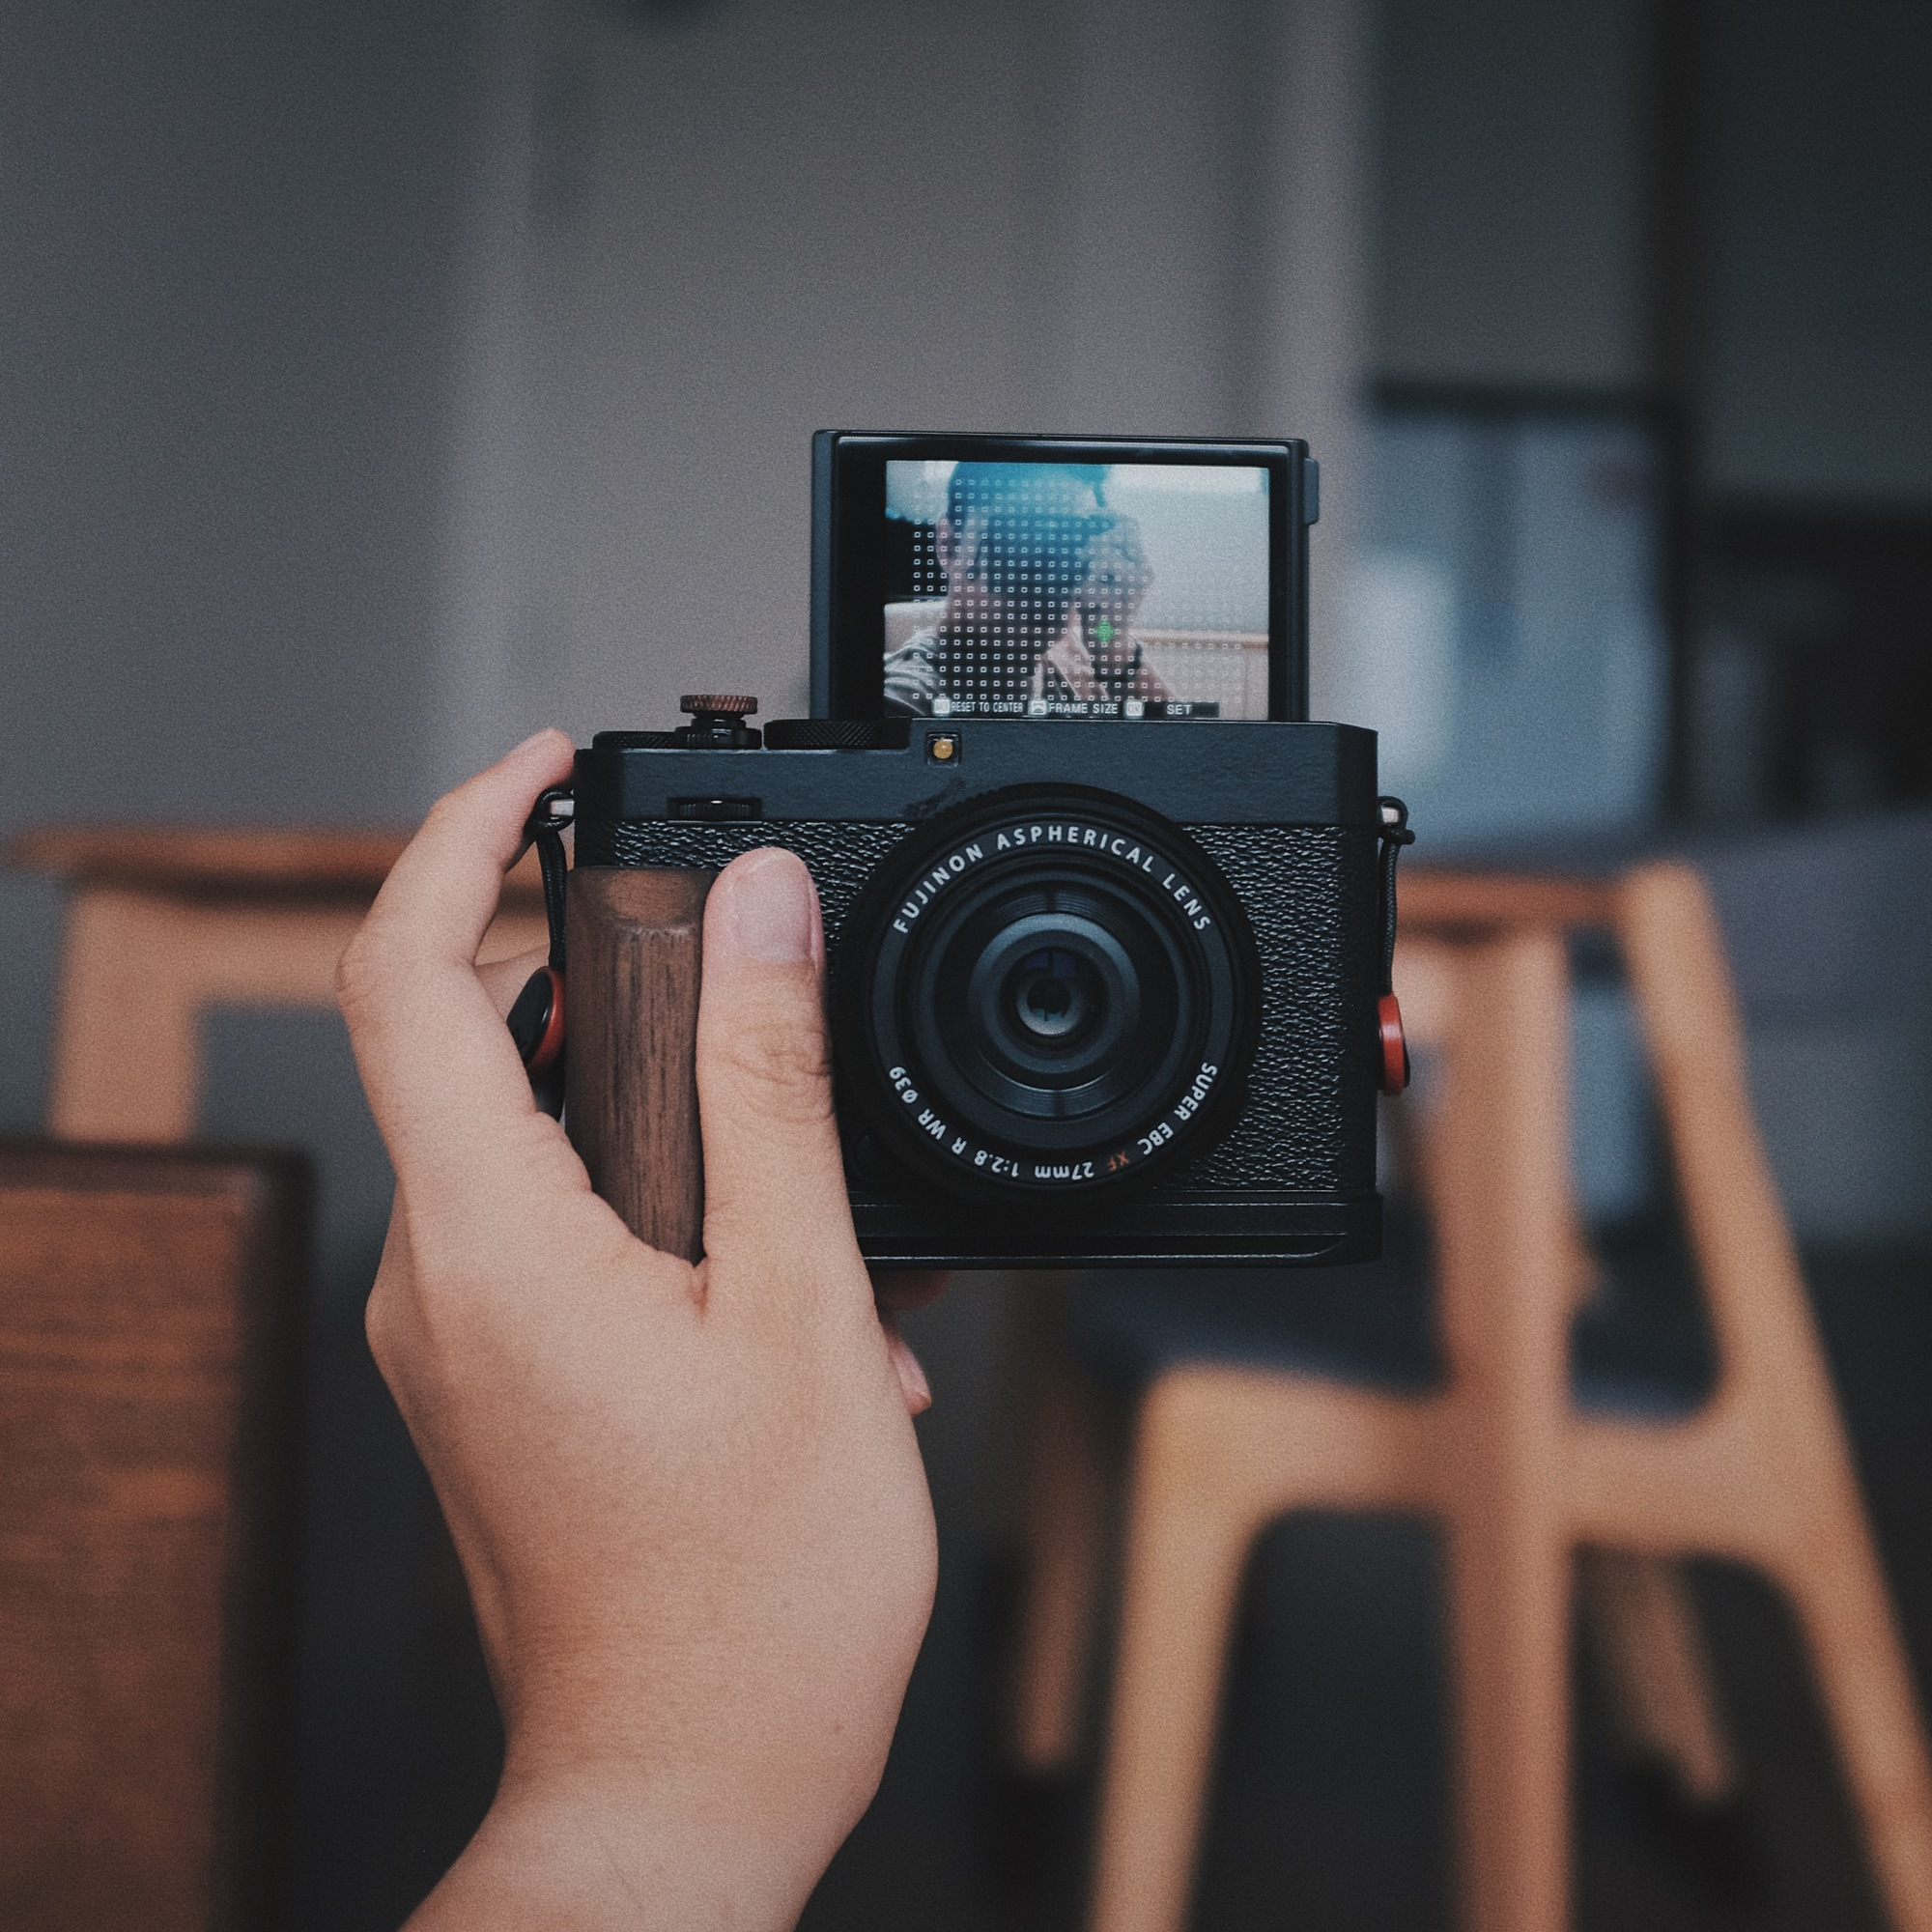
\includegraphics[width=\linewidth]{\envfinaldir/coverpic-prod.jpg}\par
            % \vskip 30pt
            \vfill

            \normalsize\rmfamily\scshape
            \copyright{} The Web Digest Project \hfill\large \envdatestr
        \end{center}
    \end{titlepage}
    % \restoregeometry
}
\newcommand{\simplehref}[1]{%
    \textcolor{blue!80!green}{\href{#1}{#1}}%
}
\renewcommand{\contentsname}{\center\Huge\sffamily\bfseries Contents\par\vskip 20pt}
\newcounter{ipartcounter}
\setcounter{ipartcounter}{0}
\newcommand{\ipart}[1]{
    % \vskip 20pt
    \clearpage
    \stepcounter{ipartcounter}
    \phantomsection
    \addcontentsline{toc}{chapter}{#1}
    % \begin{center}
    %     \Huge
    %     \sffamily\bfseries
    %     #1
    % \end{center}
    % \vskip 20pt plus 7pt
}
\newcounter{ichaptercounter}
\setcounter{ichaptercounter}{0}
\newcommand{\ichapter}[1]{
    % \vskip 20pt
    \clearpage
    \stepcounter{ichaptercounter}
    \phantomsection
    \addcontentsline{toc}{section}{\numberline{\arabic{ichaptercounter}}#1}
    \begin{center}
        \Huge
        \sffamily\bfseries
        #1
    \end{center}
    \vskip 20pt plus 7pt
}
\newcommand{\entrytitlefont}[1]{\subsection*{\raggedright\Large\sffamily\bfseries#1}}
\newcommand{\entryitemGeneric}[2]{
    % argv: title, url
    \parbox{\linewidth}{
        \entrytitlefont{#1}\par\vskip 5pt
        \footnotesize\ttfamily\mdseries
        \simplehref{#2}
    }\vskip 11pt plus 11pt minus 1pt
}
\newcommand{\entryitemGithub}[3]{
    % argv: title, url, desc
    \parbox{\linewidth}{
        \entrytitlefont{#1}\par\vskip 5pt
        \footnotesize\ttfamily\mdseries
        \simplehref{#2}\par\vskip 5pt
        \small\rmfamily\mdseries#3
    }\vskip 11pt plus 11pt minus 1pt
}
\newcommand{\entryitemAp}[3]{
    % argv: title, url, desc
    \parbox{\linewidth}{
        \entrytitlefont{#1}\par\vskip 5pt
        \footnotesize\ttfamily\mdseries
        \simplehref{#2}\par\vskip 5pt
        \small\rmfamily\mdseries#3
    }\vskip 11pt plus 11pt minus 1pt
}
\newcommand{\entryitemHackernews}[3]{
    % argv: title, hnurl, rawurl
    % \parbox{\linewidth}{
    %     \entrytitlefont{#1}\par\vskip 5pt
    %     \footnotesize\ttfamily\mdseries
    %     \simplehref{#3}\par
    %     \textcolor{black!50}{\href{#2}{#2}}
    % }\vskip 11pt plus 11pt minus 1pt
    \begin{minipage}{\linewidth}
            \entrytitlefont{#1}\par\vskip 5pt
            \footnotesize\ttfamily\mdseries
            \simplehref{#3}\par
            \textcolor{black!50}{\href{#2}{#2}}
    \end{minipage}\par\vskip 11pt plus 11pt minus 1pt
}







\begin{document}

\makeheader

\tableofcontents\clearpage




\ipart{Developers}
\ichapter{Hacker News}
\entryitemTwoLinks{Mystical}{https://news.ycombinator.com/item?id=44016037}{https://suberic.net/~dmm/projects/mystical/README.html}

\entryitemTwoLinks{Dead Stars Don't Radiate}{https://news.ycombinator.com/item?id=44015872}{https://johncarlosbaez.wordpress.com/2025/05/17/dead-stars-dont-radiate-and-shrink/}

\entryitemTwoLinks{How to have the browser pick a contrasting color in CSS}{https://news.ycombinator.com/item?id=44015367}{https://webkit.org/blog/16929/contrast-color/}

\entryitemTwoLinks{If nothing is curated, how do we find things}{https://news.ycombinator.com/item?id=44015144}{https://tadaima.bearblog.dev/if-nothing-is-curated-how-do-we-find-things/}

\entryitemTwoLinks{Proton threatens to quit Switzerland over new surveillance law}{https://news.ycombinator.com/item?id=44014808}{https://www.techradar.com/vpn/vpn-privacy-security/we-would-be-less-confidential-than-google-proton-threatens-to-quit-switzerland-over-new-surveillance-law}

\entryitemTwoLinks{Palette lighting tricks on the Nintendo 64}{https://news.ycombinator.com/item?id=44014587}{https://30fps.net/pages/palette-lighting-tricks-n64/}

\entryitemTwoLinks{O2 VoLTE: locating any customer with a phone call}{https://news.ycombinator.com/item?id=44014046}{https://mastdatabase.co.uk/blog/2025/05/o2-expose-customer-location-call-4g/}

\entryitemTwoLinks{Pyrefly: A new type checker and IDE experience for Python}{https://news.ycombinator.com/item?id=44013913}{https://engineering.fb.com/2025/05/15/developer-tools/introducing-pyrefly-a-new-type-checker-and-ide-experience-for-python/}

\entryitemTwoLinks{Push Ifs Up and Fors Down}{https://news.ycombinator.com/item?id=44013157}{https://matklad.github.io/2023/11/15/push-ifs-up-and-fors-down.html}

\entryitemTwoLinks{Catalog of Novel Operating Systems}{https://news.ycombinator.com/item?id=44012615}{https://github.com/prathyvsh/os-catalog}

\entryitemTwoLinks{JavaScript's New Superpower: Explicit Resource Management}{https://news.ycombinator.com/item?id=44012227}{https://v8.dev/features/explicit-resource-management}

\entryitemTwoLinks{A kernel developer plays with Home Assistant}{https://news.ycombinator.com/item?id=44011669}{https://lwn.net/SubscriberLink/1017720/7155ecb9602e9ef2/}

\entryitemTwoLinks{Behind Silicon Valley and the GOP's campaign to ban state AI laws}{https://news.ycombinator.com/item?id=44011654}{https://www.bloodinthemachine.com/p/de-democratizing-ai}

\entryitemTwoLinks{XTool – Cross-platform Xcode replacement}{https://news.ycombinator.com/item?id=44011515}{https://github.com/xtool-org/xtool}

\entryitemTwoLinks{Wow@Home – Network of Amateur Radio Telescopes}{https://news.ycombinator.com/item?id=44011489}{https://phl.upr.edu/wow/outreach}

\entryitemTwoLinks{A kernel developer plays with Home Assistant}{https://news.ycombinator.com/item?id=44011381}{https://lwn.net/SubscriberLink/1017720/7155ecb9602e9ef2/}

\entryitemTwoLinks{Will AI systems perform poorly due to AI-generated material in training data?}{https://news.ycombinator.com/item?id=44010705}{https://cacm.acm.org/news/the-collapse-of-gpt/}

\entryitemTwoLinks{Moody's strips U.S. of triple-A credit rating}{https://news.ycombinator.com/item?id=44009999}{https://www.ft.com/content/e456ea34-c6ad-43fe-abe9-d4ce781c07b4}

\entryitemTwoLinks{Getting AI to write good SQL}{https://news.ycombinator.com/item?id=44009848}{https://cloud.google.com/blog/products/databases/techniques-for-improving-text-to-sql}

\entryitemTwoLinks{ClojureScript 1.12.42}{https://news.ycombinator.com/item?id=44009464}{https://clojurescript.org/news/2025-05-16-release}\ichapter{Phoronix}
\entryitemGeneric{\hskip 0pt{}AMD Zen 6 Feature Flag Merged For Linux 6.15}{https://www.phoronix.com/news/AMD-Zen-6-Flag-Linux-6.15}

\entryitemGeneric{\hskip 0pt{}Debian 12.11 Pulls In Dozens Of Fixes}{https://www.phoronix.com/news/Debian-12.11-Released}

\entryitemGeneric{\hskip 0pt{}Niri 25.05 Brings New Features To This Innovative Wayland Compositor}{https://www.phoronix.com/news/Niri-25.05-Released}

\entryitemGeneric{\hskip 0pt{}KDE Plasma 6.4 Introducing An HDR Calibration Wizard}{https://www.phoronix.com/news/KDE-Plasma-6.4-HDR-Calibrate}

\entryitemGeneric{\hskip 0pt{}Debian Installer Trixie RC 1 Adds Rescue Support On Btrfs, Upgraded Linux 6.12 Kernel}{https://www.phoronix.com/news/Debian-Installer-Trixie-RC1}

\entryitemGeneric{\hskip 0pt{}NVIDIA Upstreams Newer GSP Firmware For Open-Source Nouveau Driver}{https://www.phoronix.com/news/NVIDIA-GSP-RM-570-Firmware}

\entryitemGeneric{\hskip 0pt{}FreeBSD 14.3 Beta 3 Brings KDE Plasma 6 Packages To The DVD ISOs}{https://www.phoronix.com/news/FreeBSD-14.3-Beta-3}

\entryitemGeneric{\hskip 0pt{}Rockchip Open-Source NPU Driver "RKNN" Continues Making Progress}{https://www.phoronix.com/news/Rockchip-NPU-Driver-RKNN-2025}

\entryitemGeneric{\hskip 0pt{}Intel ISPC 1.27 Released With AVX10.2 Support}{https://www.phoronix.com/news/Intel-ISPC-1.27}\ichapter{Dribbble}
\entryitemGeneric{\hskip 0pt{}DICH™ Fashion}{https://dribbble.com/shots/26032014-DICH-Fashion}

\entryitemGeneric{\hskip 0pt{}Profile Card 👧}{https://dribbble.com/shots/26033069-Profile-Card}

\entryitemGeneric{\hskip 0pt{}East Meats West}{https://dribbble.com/shots/26027917-East-Meats-West}

\entryitemGeneric{\hskip 0pt{}Assist Logo Design (Unused for Sale)}{https://dribbble.com/shots/26027053-Assist-Logo-Design-Unused-for-Sale}

\entryitemGeneric{\hskip 0pt{}Goldfish Concept}{https://dribbble.com/shots/26029115-Goldfish-Concept}

\entryitemGeneric{\hskip 0pt{}Type Illustration}{https://dribbble.com/shots/26023946-Type-Illustration}

\entryitemGeneric{\hskip 0pt{}Web3 crypto hero section 3d motion design}{https://dribbble.com/shots/26017311-Web3-crypto-hero-section-3d-motion-design}

\entryitemGeneric{\hskip 0pt{}Recent Marks \& Lettermarks}{https://dribbble.com/shots/26023308-Recent-Marks-Lettermarks}

\entryitemGeneric{\hskip 0pt{}B2B Dashboard \& Web App UI UX Design for Carbon Solutions}{https://dribbble.com/shots/25993068-B2B-Dashboard-Web-App-UI-UX-Design-for-Carbon-Solutions}

\entryitemGeneric{\hskip 0pt{}Cat and Dog Brand Mascots}{https://dribbble.com/shots/26023569-Cat-and-Dog-Brand-Mascots}

\entryitemGeneric{\hskip 0pt{}Apefilm logo}{https://dribbble.com/shots/26021962-Apefilm-logo}

\entryitemGeneric{\hskip 0pt{}UX Logo Icon Concept}{https://dribbble.com/shots/26018312-UX-Logo-Icon-Concept}

\entryitemGeneric{\hskip 0pt{}Dublo - Logo Design}{https://dribbble.com/shots/26017446-Dublo-Logo-Design}

\entryitemGeneric{\hskip 0pt{}@bitcoin website}{https://dribbble.com/shots/26005022--bitcoin-website}

\entryitemGeneric{\hskip 0pt{}DropX // Website}{https://dribbble.com/shots/26017012-DropX-Website}

\entryitemGeneric{\hskip 0pt{}Crypto Portfolio Tracker App}{https://dribbble.com/shots/26017408-Crypto-Portfolio-Tracker-App}

\entryitemGeneric{\hskip 0pt{}GrowLabs}{https://dribbble.com/shots/26017087-GrowLabs}

\entryitemGeneric{\hskip 0pt{}Trackwallet}{https://dribbble.com/shots/26013877-Trackwallet}

\entryitemGeneric{\hskip 0pt{}Coffee Brand Redesigns}{https://dribbble.com/shots/26012543-Coffee-Brand-Redesigns}

\entryitemGeneric{\hskip 0pt{}Data Wollet Logo Concept}{https://dribbble.com/shots/26013441-Data-Wollet-Logo-Concept}

\entryitemGeneric{\hskip 0pt{}D\&D stuff}{https://dribbble.com/shots/26011464-D-D-stuff}

\entryitemGeneric{\hskip 0pt{}Branding for AURA — your personal AI assistant}{https://dribbble.com/shots/26010311-Branding-for-AURA-your-personal-AI-assistant}

\entryitemGeneric{\hskip 0pt{}Enfinity Wordmark}{https://dribbble.com/shots/26013368-Enfinity-Wordmark}

\entryitemGeneric{\hskip 0pt{}Mobile App UI – Art Showcase Motion}{https://dribbble.com/shots/26011341-Mobile-App-UI-Art-Showcase-Motion}


\ipart{Developers~~~~(zh-Hans)}
\ichapter{Solidot}
\entryitemGeneric{\hskip 0pt{}特朗普要求苹果停止在印度扩大制造业务}{https://www.solidot.org/story?sid=81316}

\entryitemGeneric{\hskip 0pt{}中国二氧化碳排放首次在电力需求增长的情况下下降}{https://www.solidot.org/story?sid=81315}

\entryitemGeneric{\hskip 0pt{}太空计算卫星星座发射首批 12 颗卫星}{https://www.solidot.org/story?sid=81314}

\entryitemGeneric{\hskip 0pt{}研究发现无论是否运动久坐会损害大脑}{https://www.solidot.org/story?sid=81313}

\entryitemGeneric{\hskip 0pt{}研究发现 AI 无法预测股市}{https://www.solidot.org/story?sid=81312}

\entryitemGeneric{\hskip 0pt{}年轻恒星系统发现结晶水冰}{https://www.solidot.org/story?sid=81311}

\entryitemGeneric{\hskip 0pt{}Rust 庆祝十周年,发布 Rust 1.87}{https://www.solidot.org/story?sid=81310}

\entryitemGeneric{\hskip 0pt{}史前人类如何从北亚向北美和南美扩张}{https://www.solidot.org/story?sid=81309}

\entryitemGeneric{\hskip 0pt{}首例定制基因编辑疗法治愈婴儿的罕见遗传病}{https://www.solidot.org/story?sid=81308}

\entryitemGeneric{\hskip 0pt{}植物遇险如何通知邻居?}{https://www.solidot.org/story?sid=81307}

\entryitemGeneric{\hskip 0pt{}物理学家计算出宇宙最后一批恒星将在 10^78 年后彻底死亡}{https://www.solidot.org/story?sid=81306}

\entryitemGeneric{\hskip 0pt{}欧盟指责 TikTok 广告不透明}{https://www.solidot.org/story?sid=81305}

\entryitemGeneric{\hskip 0pt{}Red Hat Enterprise Linux 10 GA}{https://www.solidot.org/story?sid=81304}

\entryitemGeneric{\hskip 0pt{}研究发现 ChatGPT 降低了头脑风暴中的创意多样性}{https://www.solidot.org/story?sid=81303}

\entryitemGeneric{\hskip 0pt{}长时间工作可能会改变大脑结构}{https://www.solidot.org/story?sid=81302}

\entryitemGeneric{\hskip 0pt{}火星首次观测到可光见波段的绿色极光}{https://www.solidot.org/story?sid=81301}

\entryitemGeneric{\hskip 0pt{}印度在其境内屏蔽 X 的新华社账号}{https://www.solidot.org/story?sid=81300}

\entryitemGeneric{\hskip 0pt{}xAI 的 Grok 突然不停的说南非``白人种族灭绝''''}{https://www.solidot.org/story?sid=81299}

\entryitemGeneric{\hskip 0pt{}朝鲜黑客组织使用俄罗斯网络基础设施发动攻击}{https://www.solidot.org/story?sid=81298}

\entryitemGeneric{\hskip 0pt{}华纳兄弟探索的流媒体服务 Max 恢复原名 HBO Max}{https://www.solidot.org/story?sid=81297}\ichapter{V2EX}
\entryitemGeneric{\hskip 0pt{}[问与答] 想不出来下周吃什么怎么办?}{https://www.v2ex.com/t/1132491}

\entryitemGeneric{\hskip 0pt{}[生活] 恋爱三年已订婚,女友觉得我长得丑决定分手}{https://www.v2ex.com/t/1132490}

\entryitemGeneric{\hskip 0pt{}[硬件] 电子白板的技术实现}{https://www.v2ex.com/t/1132488}

\entryitemGeneric{\hskip 0pt{}[分享发现] 风鸟 查企业 注册送 5 年 SVIP 赶快注册}{https://www.v2ex.com/t/1132487}

\entryitemGeneric{\hskip 0pt{}[分享发现] 大家有学第二门外语的吗?}{https://www.v2ex.com/t/1132486}

\entryitemGeneric{\hskip 0pt{}[Apple] [求助] 有人遇到 Mac WiFi 断流问题吧}{https://www.v2ex.com/t/1132485}

\entryitemGeneric{\hskip 0pt{}[程序员] 用 kong 做网关, https 协议下页面每隔一秒刷新一次}{https://www.v2ex.com/t/1132484}

\entryitemGeneric{\hskip 0pt{}[问与答] 咨询一下,有没有会写电报(TG)小程序的,付费做项目,谢谢}{https://www.v2ex.com/t/1132483}

\entryitemGeneric{\hskip 0pt{}[程序员] 30 岁了,感觉干运维开发没有出路,没有未来}{https://www.v2ex.com/t/1132482}

\entryitemGeneric{\hskip 0pt{}[程序员] 值夜班后遗症,作息乱了}{https://www.v2ex.com/t/1132480}

\entryitemGeneric{\hskip 0pt{}[酷工作] 下一代开源可编程 GenAI 平台寻找合作开发者}{https://www.v2ex.com/t/1132479}

\entryitemGeneric{\hskip 0pt{}[NAS] 有没有用来做冷备的硬盘推荐}{https://www.v2ex.com/t/1132477}

\entryitemGeneric{\hskip 0pt{}[问与答] openrouter 的价格计算到底是什么逻辑有人知道吗?}{https://www.v2ex.com/t/1132476}

\entryitemGeneric{\hskip 0pt{}[酷工作] 招聘 | AWS + Kubernetes + ArgoCD + Github CI/CD 开发顾问}{https://www.v2ex.com/t/1132475}

\entryitemGeneric{\hskip 0pt{}[问与答] 有没有可以免费取消的机票啊?}{https://www.v2ex.com/t/1132473}

\entryitemGeneric{\hskip 0pt{}[Apple] IOS18.4 的相册更新,有人能 get 到吗?从安卓转苹果被恶心了好几年的功能缺失,终于做了}{https://www.v2ex.com/t/1132471}

\entryitemGeneric{\hskip 0pt{}[Android] idm 嗅探到了视频源但要手动点击下载,能否自动化下载?}{https://www.v2ex.com/t/1132470}

\entryitemGeneric{\hskip 0pt{}[程序员] 刚刚听用谷歌的 notellm 生成的播客,他给我留下一个很有意思的思考}{https://www.v2ex.com/t/1132468}

\entryitemGeneric{\hskip 0pt{}[分享创造] 一个工具,能搬运 X 的推文,利用 AI 二次创作}{https://www.v2ex.com/t/1132467}

\entryitemGeneric{\hskip 0pt{}[问与答] Mac 扩容}{https://www.v2ex.com/t/1132466}

\entryitemGeneric{\hskip 0pt{}[问与答] 论坛的 2FA 被小孩直接删掉了,怎么办?}{https://www.v2ex.com/t/1132464}

\entryitemGeneric{\hskip 0pt{}[分享发现] 软件代理的思考}{https://www.v2ex.com/t/1132463}

\entryitemGeneric{\hskip 0pt{}[生活] 今天在公园目睹一场霸凌}{https://www.v2ex.com/t/1132462}

\entryitemGeneric{\hskip 0pt{}[NAS] 新版 Plex App 屎一样的难用没人吐槽么}{https://www.v2ex.com/t/1132460}

\entryitemGeneric{\hskip 0pt{}[户外运动] 重装徒步入门装备求推荐}{https://www.v2ex.com/t/1132459}

\entryitemGeneric{\hskip 0pt{}[程序员] 国内还有活跃的编程 UP 主吗?}{https://www.v2ex.com/t/1132458}

\entryitemGeneric{\hskip 0pt{}[分享创造] 一个失败的万年历相关的苹果 App}{https://www.v2ex.com/t/1132457}

\entryitemGeneric{\hskip 0pt{}[问与答] 想自己练羽毛球,这种训练器怎么样?}{https://www.v2ex.com/t/1132456}

\entryitemGeneric{\hskip 0pt{}[Planet] Planet 写了一个博客之后没办法运行}{https://www.v2ex.com/t/1132455}

\entryitemGeneric{\hskip 0pt{}[Apple] 美区 Apple 账户绑定了一张卡后无法兑换礼品卡?}{https://www.v2ex.com/t/1132454}

\entryitemGeneric{\hskip 0pt{}[编辑器] 随着屏幕的增大,还在限制或建议每行 80 个字符是否还合理?}{https://www.v2ex.com/t/1132453}

\entryitemGeneric{\hskip 0pt{}[程序员] 谁能帮我解决这个问题?}{https://www.v2ex.com/t/1132452}

\entryitemGeneric{\hskip 0pt{}[NAS] 设备播放杜比视界视频的问题}{https://www.v2ex.com/t/1132450}

\entryitemGeneric{\hskip 0pt{}[分享发现] 百元左右无线鼠标求推荐}{https://www.v2ex.com/t/1132449}

\entryitemGeneric{\hskip 0pt{}[问与答] 想问一下大家关于 app 的盈利方式。}{https://www.v2ex.com/t/1132448}

\entryitemGeneric{\hskip 0pt{}[酷工作] [远程][外包] 全栈或偏后端方向}{https://www.v2ex.com/t/1132447}

\entryitemGeneric{\hskip 0pt{}[问与答] 闲鱼上的(电子)产品 水深吗? 想买套 Jetson Orin Nano Super Developer Kit}{https://www.v2ex.com/t/1132446}

\entryitemGeneric{\hskip 0pt{}[macOS] macOS 多桌面下 Finder 行为混乱}{https://www.v2ex.com/t/1132445}

\entryitemGeneric{\hskip 0pt{}[Google] 为什么在未设置 robots.txt 的情况下, Google 搜索不到上海人大官方网站 www.shrd.gov.cn 的任何内容但是 Bing 却能搜索到大部分公开内容}{https://www.v2ex.com/t/1132443}

\entryitemGeneric{\hskip 0pt{}[问与答] 求手机推荐,感谢!}{https://www.v2ex.com/t/1132442}

\entryitemGeneric{\hskip 0pt{}[Visual Studio Code] VS Code \& Agent Dev Day,来啦!上海见}{https://www.v2ex.com/t/1132440}

\entryitemGeneric{\hskip 0pt{}[投资] 请教个期权策略}{https://www.v2ex.com/t/1132437}

\entryitemGeneric{\hskip 0pt{}[问与答] 被 OneDrive 客户端恶心到了,请求推荐一个第三方工具同步/备份本地文件夹到 OneDrive}{https://www.v2ex.com/t/1132436}

\entryitemGeneric{\hskip 0pt{}[Windows] windows 今天修复了微软拼音默认中文的问题了,可以去更新试试了}{https://www.v2ex.com/t/1132434}

\entryitemGeneric{\hskip 0pt{}[耳机] 韶音 OpenDots ONE 和 华为 free clip 选哪一个?}{https://www.v2ex.com/t/1132433}

\entryitemGeneric{\hskip 0pt{}[硬件] 坐标上海,索尼电视故障了,有靠谱的维修推荐吗?}{https://www.v2ex.com/t/1132432}

\entryitemGeneric{\hskip 0pt{}[NAS] 自己搭 Bitwarden,没有公网 ip 用 tailscale 的问题}{https://www.v2ex.com/t/1132431}

\entryitemGeneric{\hskip 0pt{}[酷工作] [上海] WEB 中级前端开发工程师(React 方向)18-22K}{https://www.v2ex.com/t/1132429}

\entryitemGeneric{\hskip 0pt{}[职场话题] 找工作遇到的免费培训包就业的情况}{https://www.v2ex.com/t/1132426}

\entryitemGeneric{\hskip 0pt{}[广州] 求一个广州靠谱的 Macbook 维修}{https://www.v2ex.com/t/1132425}


\ipart{Generic News}
\ichapter{联合早报}
\entryitemWithDescription{黎康:魔都的B面}{https://www.zaobao.com/news/china/story20250426-6241474}{``确实这几年上海的城市公共建设很好,但你有没有去看过一些老旧小区的环境?小区里电线横飞,绿化基本毫无规划;进入楼道,你会感觉回到20年前\ldots\ldots'' 上一篇``早点------沪上闲语''发表后,收到一封读者来信。这位上海市民告诉我,在装点城市门面的郁金香背后,如果走进上海的老旧小区,会看到这座城市的另一面……}

\entryitemWithDescription{新闻人间:从``不懂球的胖子''到改革推手——刘国梁}{https://www.zaobao.com/news/china/story20250426-6238850}{中国乒乓球协会星期三(4月23日)突然宣布,刘国梁主动辞去主席一职。这一消息迅速引发体坛热议,有球迷为他的离开感到惋惜,也有体育评论员开始审视他在任期内的功与过。 刘国梁自2018年起担任乒协主席,如今在第二任期尚未结束之际中途请辞,外界难免有诸多猜测。星期三当天,他以主席身份在乒协会议上作最后一次发言时,几度哽咽,甚至当场落泪。 他在记者会上透露,早在去年巴黎奥运会结束后,便已向上级表达了去意……}

\entryitemWithDescription{中国据报考虑暂停加征部分美国产品125\%关税}{https://www.zaobao.com/news/china/story20250425-6245926}{中国政府据报考虑暂停对部分美国进口产品加征125\%的关税,受访学者认为此举主要考虑中国企业的生存需要,与中美是否开启贸易谈判无关。 据彭博社引述知情人士报道,中国政府正考虑取消对美国的医疗设备,以及乙烷等工业化学品加征的报复性关税。中国是全球最大的塑料制造国,但部分工厂依赖从美国进口的乙烷。中国医院也需要美国生产的磁共振成像和超声仪器等医疗设备。 知情人士称,飞机租赁也可能豁免关税……}

\entryitemWithDescription{中国美国商会白皮书:五分之一美企不再视中国为优先投资地}{https://www.zaobao.com/news/china/story20250425-6245113}{中国美国商会的调查显示,五分之一的在华美国企业不再将中国列为优先的投资目的地。 该商会星期五(4月25日)发布由100余名中国美国商会会员企业代表共同撰写的2025年《美国企业在中国白皮书》。 白皮书指出,中美两国关系日益紧张,已连续五年成为在华美资企业面临的首要商业挑战,超过了合规风险和来自中国企业的竞争压力……}

\entryitemWithDescription{中国发布生态调查报告 称菲律宾捕捞现场发现人为弃置物}{https://www.zaobao.com/news/china/story20250425-6244616}{(北京讯)中国多家自然生态机构星期五(4月25日)联合公布一份调查报告,评估铁线礁、牛轭礁珊瑚礁的生态系统状况,称菲律宾所谓``中国在铁线礁倾倒珊瑚碎屑等言论''毫无科学和事实依据。 中国自然资源部微信公号分别发表了这份题为《铁线礁、牛轭礁珊瑚礁生态系统调查报告》的中英文版本,参与编制的机构包括中国自然资源部南海发展研究院、南海生态中心等……}

\entryitemWithDescription{香港公共场所明年起设更多禁烟区 违例罚款提高一倍}{https://www.zaobao.com/news/china/story20250425-6245064}{为了进一步降低吸烟率,香港特区政府将由明年起在更多公共场所设立禁烟区,并把违例吸烟的罚款金额提高一倍至3000港元(508新元)。 相关条例草案星期五(4月25日)刊宪,列明从明年元旦起,禁止在等候公共交通工具、等候进入电影院、医院、公众游乐场地、体育场等地方的划定范围吸烟。违者罚款由1500港元倍增至3000港元……}

\entryitemWithDescription{两韩国顶尖半导体专家 退休后被中国高校任用}{https://www.zaobao.com/news/china/story20250425-6244895}{(首尔讯)中国正通过从海外引进顶尖人才,与美国争夺高科技主导权。韩国两名``国宝级''顶尖专家退休后在本国受到冷落,未能找到合适研究职位,目前已被中国高等学府任用。 据韩国《中央日报》报道,韩国知名碳纳米管专家李永熙去年11月正式受聘于湖北工业大学半导体与量子研究所……}

\entryitemWithDescription{美国传降对陆关税又强化对台论述 分析:谈判或拿台湾当筹码}{https://www.zaobao.com/news/china/story20250425-6244227}{华盛顿释出降低对华关税信号、寻求谈判之际,美国星期三(4月23日)首次在联合国安理会批评北京误用联大2758号决议;更在同一天派遣军舰穿越台湾海峡。受访学者分析,这些作为现阶段暂与关税战没有直接关联,但不排除美国总统特朗普接下来可能利用台湾问题作为对华谈判筹码。 特朗普本周透露考虑大幅度降低对华关税,希望与中国达成``公平的协议'',同时又声称美国每天都同中国直接联系……}

\entryitemWithDescription{韩咏红:特朗普关税从``解放日''走到``妥协日''了?}{https://www.zaobao.com/news/china/story20250425-6240846}{美国总统特朗普在4月2日宣布对等关税政策,短短20天后,特朗普的高姿态已难以为继。特朗普在4月9日就已调整过一次战术,暂缓对其他国家课征对等关税,集中火力单挑中国;而今,特朗普恐怕又要眨眼了,对中国商品课征的145\%关税也可能显著下调。 特朗普近日罕见地对中国伸出橄榄枝,表示考虑大幅度降低对华关税,显露出急于与中国达成协议。但中国偏是表现得不着急……}

\entryitemWithDescription{学者:中国以2+2机制拉拢东南亚国家抗衡美国}{https://www.zaobao.com/news/china/story20250424-6240690}{受访学者分析,在中美关系因贸易战而全面恶化的大背景下,中国正以``外交、国防2+2对话机制''为新抓手,积极拉拢亚细安成员国,以抗衡美国在本区域的影响力,预计中国接下来将推动与更多区域国家建立2+2机制。 中国和印度尼西亚星期一(4月21日)在北京举行外长、防长对话机制下的首次部长级会议,两国在2023年就建立2+2对话机制。中国官方称,这是中国在全球建立的首个部长级2+2机制……}

\entryitemWithDescription{中埃空军首次联训 学者:中国初步具备向中东快速战略投送能力}{https://www.zaobao.com/news/china/story20250424-6240357}{中国空军上周派出多架战斗机、预警机、运输机与空中加油机前往埃及,进行两军首次联训。这是中国空军首次以完整作战体系进行跨洲机动。 受访学者认为,这是中国空军现代化进程的里程碑,有助于发展长途奔袭的技战术;这也标志着中国初步具备向中东进行快速战略投送的能力。 据中国国防部消息,中国与埃及两国空军于4月中旬至5月上旬,在埃及空军基地组织代号为``文明之鹰-2025''的联合训练……}

\entryitemWithDescription{台湾收紧民众申领大陆证照规定 持大陆定居证也将被撤销台湾身份}{https://www.zaobao.com/news/china/story20250424-6239789}{(台北综合讯)台湾再度收紧民众申领中国大陆证照的规定,持有大陆定居证的台湾民众也触犯相关法令,将丧失台湾身份。 综合《旺报》与《联合报》报道,台湾行政院公报显示,陆委会近日对《两岸条例》当中规定发布解释函令称,为确保两岸人员单一身份制度,两岸条例规定台湾人民不得在大陆地区``设有户籍'',或领用大陆地区护照,否则将丧失台湾身份……}

\entryitemWithDescription{神舟二十号成功发射 航天员将开展中国首次涡虫空间再生实验}{https://www.zaobao.com/news/china/story20250424-6239950}{(北京综合讯)中国星期四(4月24日)成功发射神舟二十号载人飞船。三名航天员将在空间站驻留约六个月,并开展中国首次涡虫空间再生实验。 综合新华社、央视新闻和《中国青年报》报道,搭载神舟二十号的长征二号F遥二十运载火箭,星期四下午5时17分在甘肃酒泉卫星发射中心点火发射。约10分钟后,神舟二十号与火箭成功分离,进入预定轨道……}

\entryitemWithDescription{台大罢免升温 朝野对抗加剧}{https://www.zaobao.com/news/china/story20250424-6240062}{台湾两大在野党将携手举办大型造势活动,抗议政府利用司法整肃异己,进行大罢免。兼任民进党主席的总统赖清德则公开肯定公民团体罢免在野党立委的行动影片,检调也持续搜索在野国民党宜兰县党部,朝野对抗情势正逐步升温……}

\entryitemWithDescription{美国国会罕见动用传唤权 调查中国三电信巨头}{https://www.zaobao.com/news/china/story20250424-6239456}{(纽约路透电)美国众议院中国问题特别委员会星期三(4月23日)罕见地动用传唤权,调查中国三大电信公司涉嫌支持中国军方和政府的行为。 据路透社报道,中国移动、中国电信和中国联通三家中国电信巨头收到该委员会的传唤通知,须回答他们是否可通过在美开展的云服务和互联网业务获取美国数据的问题。 美国两党议员持续对被指由中国主导的网络攻击事件表示担忧……}

\entryitemWithDescription{浙江一小学门外发生汽车冲撞人群事件}{https://www.zaobao.com/news/china/story20250424-6238514}{(香港综合讯)中国再发生校园伤人事件,浙江金华一所小学门外星期二(4月22日)放学时有汽车冲撞人群,伤亡人数不明。官方在事发两日后仍未发布通报,中国社媒上的相关信息均被删除。 综合《明报》《南华早报》和网媒``香港01''报道,这起事件发生在金华市苏孟乡中心小学门口,时间是星期二傍晚5时45分左右,正值放学时间。附近商户披露,有多名学生被撞……}

\entryitemWithDescription{学者:关税战伤敌一千自损八百 中美终将找到共处之道}{https://www.zaobao.com/news/china/story20250424-6238821}{美国总统特朗普祭出对等关税将届满一个月,如今传出可能降低对华关税,定居美国的资深华人学者赵全胜指出,中美领导阶层有一批人长期相信对方马上要垮台,但关税战让双方意识到,这无疑是``伤敌一千,自损八百'',因此迟早会找到共处之道。 特朗普4月2日宣布全面实施对等关税,随后在9日紧急暂缓90天,让各国争取与美国谈判的时间与空间,唯独对中国不断加码;北京也不甘示弱,提出相应反制……}

\entryitemWithDescription{打击电诈犯罪扩至纵深地带 缅甸向中国移交920余名嫌犯}{https://www.zaobao.com/news/china/story20250424-6238307}{(北京综合讯)中国与缅甸加大打击电信网络诈骗犯罪合作力度,两国最近一个月的合作执法行动,已从缅北地区扩大到当阳、勐休等缅甸纵深地带。 中国公安部官网星期三(4月23日)通报,缅甸执法部门近日将在当地抓获的920余名中国籍涉诈犯罪嫌疑人,通过云南西双版纳打洛口岸全部移交中国警方。 通报称,缅北电诈犯罪集团遭受重创,但部分涉诈人员为逃避打击,向当阳、勐休等纵深地带转移藏匿,继续实施跨境电诈……}

\entryitemWithDescription{沈泽玮:魔幻山城的中国式现代化演绎}{https://www.zaobao.com/news/china/story20250424-6234868}{时隔12年因工作再访重庆,春夏交替之际迎来烈日当空,与当年冬季旅游行走于山城迷雾的印象截然不同。 5000架无人机灯光秀,既展现科技力量也打造视觉盛宴;科企创始人讲述营商环境不断优化;村委会主任手捧涪陵榨菜分享东方酱腌菜``走出去''成果;火车司机传递通关速度如何带动互联互通跨境贸易;公安局交巡警总队科研处综合科科长讲述数字化赋能超大城市治理;社区党委书记分享中国特色``民主村''的前身今世……}

\entryitemWithDescription{中国网购平台将全面取消``仅退款''}{https://www.zaobao.com/news/china/story20250423-6234242}{在中国官方整治``内卷式竞争''的背景下,中国电商平台将全面取消``仅退款''选项。受访学者认为,此举有助行业回归良性竞争,是对电商市场的一次纠偏。 据《北京商报》报道,拼多多、淘宝、抖音、快手、京东等多个中国电商平台,星期二(4月22日)修改有关``仅退款''的相关条款,消费者申请``退款不退货'',将由商家自主处理……}

\entryitemWithDescription{3月人民币跨境收付占比刷新历史纪录}{https://www.zaobao.com/news/china/story20250423-6233857}{(华盛顿彭博电)随着美元的全球吸引力减弱、中美贸易紧张局势上升,3月中国投资者和贸易公司在国际结算中对人民币的使用大幅增加,创下历史纪录。 彭博社基于中国国家外汇管理局星期二(4月22日)公布的数据计算,3月中国大陆境内个人和机构的跨境业务中,人民币使用占比达 54.3\%,总额7249亿美元(9502亿新元)……}






\clearpage
\leavevmode\vfill
\footnotesize

Copyright \copyright{} 2023-2025 Neruthes and other contributors.

This document is published with CC BY-NC-ND 4.0 license.

The entries listed in this newsletter may be copyrighted by their respective creators.

This newsletter is generated by the Web Digest project.

The newsletters are also delivered via Telegram channel \CJKunderline{\href{https://t.me/webdigestchannel}{https://t.me/webdigestchannel}}.\\
RSS feed is available at \CJKunderline{\href{https://webdigest.pages.dev/rss.xml}{https://webdigest.pages.dev/rss.xml}}.

This newsletter is available in PDF at
\CJKunderline{\href{https://webdigest.pages.dev/}{https://webdigest.pages.dev/}}.

The source code being used to generate this newsletter is available at\\
\CJKunderline{\href{https://github.com/neruthes/webdigest}{https://github.com/neruthes/webdigest}}.

This newsletter is also available in
\CJKunderline{\href{http://webdigest.pages.dev/readhtml/\envyear/WebDigest-20250518.html}{HTML}} and
\CJKunderline{\href{https://github.com/neruthes/webdigest/blob/master/markdown/\envyear/WebDigest-20250518.md}{Markdown}}.


\coverpic{https://unsplash.com/photos/waves-on-the-ocean-surface-sparkle-in-the-sunlight-BPHyN1U\_ci8}{Barbare Kacharava}


\end{document}
